%
\section{Grouping and labeling}
%
% Remember to mention that video quality isn't used after phase 1 due to the side effects cased by labeling the video (namely that bad quality segments don't receive any labels). in a real world application this quality measure could be used to reduce the amount of data to analyze
Grouping and labeling comes down to extracting information about what is happening in a piece of video footage. We want to be able to distinguish between different \textit{types} of scenes so we have a way to construct final videos using a \textit{recipe} of some sort. This recipe would define what kinds of clips we want in the video and in what order they should appear.
%
\subsection{Literature Study}
%
% Noter fra Kim: Mangler noget i denne sektion
%
%Lauge:
There are many ways to extract context from images, sound and video. Some focus on the depicted scene itself, while others look at the events happening in the scene. Location and time of day would be an example of the former while elements such as excitement, violence and other specific behaviour are examples of the later.\\
Hanjalic, A. For example, \cite{citeulike:405480} describes a way to identify regions of high levels of excitement in sports video-clips based on a manually selected set of features. These features can be both visuals (like the movement in an image or the change of camera positions) or audial (namely the energy contained in the audio track).\\
Optical Flow, as described by Bouguet \cite{Bouguet2000}, can also be used to detect events or objects in video. Optical Flow looks at how objects move around by tracking a collection of points across frames in a video.
Reisman et. al. \cite{CrowdDetectionInVideoSequences} describes a way to identify crowds from a moving vehicle by looking for inward moving optical flow.
Optical flow
Day Night Classification
Crowd detection
\\
%
%Anders:
% describe Haar cascade classifiers (performance and an outline of how they work)
With the introduction of Haar cascade classifiers by Viola and Jones\cite{viola01}, later improved upon by Lienhart and Maydt\cite{lienhart01} and by Schmidt and Kasinski\cite{schmidt01}\cite{schmidt02}, there exists a very efficient tool for facial detection.
% anything on police detection (maybe violence detection)? crowd detection? 
%
\subsection{Method}
%
method...
%
\subsection{Metadata}
%
Before we attempt to label the content in the videos we first extract all the metadata we can. MOOOORE....
%
\subsubsection{Facial Detection}
%
OpenCV provides an implementation of an already trained classifier, manifested as a range of xml-files describing the Haar like features of a human face, both front and profile, aswell as upper body, lower body, and full body (CONFIRM!!!!!).\\
%
% Noter fra Kim: Yes, i det mindste nogle flere detaljer
%
The Haar Cascade Classifier (HCC) uses a data-structure called an integral image, an algorithm based on AdaBoost that selects critical visual features, and a method that combines complex classifiers to compute on the most promising object-like regions.\\
An integral image is a matrix where any point $(x,y$ is the sum of all pixels above and to the left of $(x,y)$. Not only is the computation of this matrix efficient as a function of its nature (it can reuse already computed sums when building the matrix), the sum at any given point can be computed in constant time as it can be done by 4 lookups in the matrix followed by 4 additions and substractions. A FIGURE WOULD ILLUSTRATE THIS QUITE WELL.\\
%
% Noter fra Kim: YEP
%
AdaBoost (Adaptive Boosting) is a meta-algorithm for boosting machine learning algorithms where subsequent classifiers built are tweaked in favor of those instances misclassified by previous classifiers (partly FROM WIKI). The derivative algorithm is a modification of AdaBoost that constrains each returned (weak) classifier to be dependent only on a single feature, which in turn is deemed a critical feature.\\
A method of using less complex processing to detect promising regions, and then apply the more complex processing on these regions.\\
OpenCV provides a python-implementation of an already trained Haar cascade classifier, manifested as a range of xml-files describing the Haar like features of a human face, both front and profile, aswell as upper body, lower body, and full body.\\
By deploying facial detection to every frame in each video we get a good estimate of how many people are present, and also their location within each frame. This estimate is limited by the quality of the frame, ie. shaky video-clips have a reduced detection rate, and we also experienced a significant increase in false positives for banners and flags (which there is a presence well above normal, compared to most other types of video footage).\\
Initial measurements by Viola achives 15 frames per second detection in an 384 by 288 pixel image on, by todays standards, outdated hardware, we are working with 480 by 640 pixel images, an almost 3 times larger area, we still had close to real-time facial detection (working on video with 24 frames per second). This is however not practical if a computer had to analyze multiple video-streams (as in our case). For the sake of simplicity we did not perform the obvious optimization of only analayzing select frames (ex. every third frame). Analyzing all of our footage was still done overnight, but as we interpolate the results afterswards, we would not expect these to suffer much from the before-mentioned optimization.\\
We suggest that further optimizations involve exploiting the ready-at-hand metadata such as the general frame quality which severely impacts facial detection rates in a negative fashion.\\
A more advanced optimization would be to exploit the temporal data achived when analyzing frame-by-frame. Ie. we could exploit knowledge gained in previous frames to speed up human detection in subsequent frames.

%
\subsubsection{Brightness}
%
The brightness of a video is expressed as an array of means
%
% Noter fra Kim: Hvorfor et array? Er det ment som en funktion af tid/frame (brug ikke implementations sprog)
%
of the color intensity through all frames in the video. Since the videos have already been converted to grayscale at this point in the pipe-line this is a trivial task, due to there only being a gray channel in the pixels.
%
\subsubsection{Optical Flow}
%
% TODO: Move this section below Shift Vector Magnitude
%
% TODO: Describe Optical Flow in general
%
Our experiments with Optical Flow are based on a wish to extract information about what is happening in the video. Whereas the Shift Vector Magnitude tells us something about how the camera itself moves, Optical Flow attempts to explain how the content within each frame moves. There has been a substancial amount of research put into this field. [REFS] describes ways to identify certain types of actions occuring within videos, such as violent behaviour, [REF] looks at general crowd movement in public places, and Reisman et. al. \cite{CrowdDetectionInVideoSequences} describes how Optical Flow can be used to identify pedestrians, even at great distance where such methods as Facial- and People- Detection come up short.\\
%
One huge difference between our work and that of all the previous research we have been able to find is that we do not have the luxary of a stationary camera, or, in the case of the pedestrian detection \cite{CrowdDetectionInVideoSequences}, at least a fixed camera.
%
% Noter fra Kim: What? Knowing the camera motion(?)
%
Most of our footage is recorded by handheld cameras often under very poor conditions. Extracting the optical flow of our videos is therefore not only a matter of analysing how reference points move around in the frame. First we need to \textit{stabilise} the frame itself.\\
%
% Noter fra Kim:  Missing a definition: Optical Flow = Changes in the intesinty pattern. Indirectly changes in the 3D scene
%
%
\paragraph{Frame stabilisation}
%
There are several obvious ways to do this, but each has its own limitations. The first that comes to mind is to simply use the Shift Vector Magnitudes that we have already computed. This intuitively makes a lot of sense since they are suppose to tell us something about how the camera moves at each point of the video. Thus, it should simply be a matter of subtracting this general movement from whatever individial movement is detected within the frame and the remaining movement would be the optical flow of the content. However, it turns out that although the Shift Vector approach is very suitable for describing the general type of cameara movement (shaking, panning), especially when the data is smoothed across several frames, it has a relatively high margin of error for individual frames. This is especially the case if the camera moves very fast or if there actually \textit{is} a lot of movement within the frame. Other approaches [REF] involve calculating the optical flow and then subsequently subtracting the mean of all the individual vectors it yields, from the each of the vectors.
%
% Noter fra Kim: Knudret sætning
%
Yet another way [REF] is to detect the most dominant vector direction and use that as a stabiliser. However, all our experimentation showed that these methods suffer from one serious limitaion. If moving objects in the frame a very close to the camera, they tend to become more influencial than the stationary background and they end up swapping roles. The very movement we want to extract is removed and everything we would like to get rid of remains. The border-case for this condition is especially problematic. This occurs when an object is at the exact distance from the the camera where it \textit{periodically} becomes the dominant set of movement. In these cases the stabilising vector will jump from one extreme to the other and thus be completely useless.\\
Some of these problems could probably be alleviated through further analysis or averaging across time, however, through our experimentation we came up with an approach that seems quite promising.\\\\
%
We noticed that a preliminary detection of Good Features to Track was very beneficial. The method, described by [REF] is based around detecting pixels (or \textit{corners}) in an image, that has high eigenvalues.
%
% Noter fra Kim: Eigenvalues of what? Hessian matrix (second order derivatives)? How do you use these points?
%
These points has a tendency to be present in stationary objects in the frame far more often than in moving objects, and thus form a very decent base for our stabilising vector. We chose to calculate the mean of these vectors and use that, although it also would be possible to detect the most common direction as described above and in [REF].
%
\paragraph{Detecting movement}
%
With the frame itself stabilised it is possible to analyse the movement within it. We do this by placing a grid of points across the frame and then feed these points to an Optical Flow algorithm, more specifically a pyramidal implementation of the Lucas Kanade feature tracker described by Bouguet \cite{Bouguet2000}. We do the analysis with a grid of 24x16 points, using a search window of 30x30 pixels through two iterations.\\% TODO: ACTUALLY UNDERSTAND THIS!!!
Some of the resulting vectors are considered invalid if the algorithm is unable to track them (this is often the case with points in the sky or in surfaces without any distinct features), if the algorithm estimate a too large margin of error, or if the point being tracked ends up outside of the subsequent frame. For the rest, we then subtract the stabilising vector we computed earlier from each them. The result should (at least in theory) be a set of vectors describing how different parts of the image move in relation to each other. For simplicty we group these vectors into nine groups each representing one of nine boxes each covering their own part of the frame.
%
% Noter fra Kim: Figure
%
An average movement and the average length of all movements are calculated for each box and these nine vectors are stored for each frame.
%
% TODO: Write a bit more about how these nine vectors tells us how objects in that part of the image generally moves
%
% REMEMBER: Describe RISKS (zooming)
\subsubsection{Blue channel}\label{sec:blue_channel}
%
Each frame in a video consists of a matrix of pixels in 3 channels, red, green, and blue. For the purpose of police detection, described in detail in section \ref{sec:police_detection}, and day/night detection, described in detail in section \ref{blah}, we extracted the blue channel in each frame and computed the mean pixel intensity.
%
\subsubsection{Contrast}
%
Some of the metadata is already extracted in earlier phases. The contrast is an example of this. The contrast in a frame is defined as being the standard deviation of the intensity values in the image-matrix. A small deviation would indicate little contrast/diversity in color-intensity, and a large deviation would indicate a high contrast/much diversity in intensity. Again, the contrast metadata for each video is expressed as an array of these standard deviations in each frame.
%
\subsubsection{Shift Vector Magnitude}
%
Like the contrast, the shift vector magnitudes for each video is already computed as a part of the initial image quality assessment. We attempt to estimate the camera movement by \textit{shifting} each frame until its content more or less alligns with the content of the previous frame. This shift is expressed as a vector, whos magnitude tells us how much the camera is moving/shaking at each frame point in the video.
%
\subsection{Labels}
%

%
\subsubsection{Police Detection}\label{sec:police_detection}
%
By investigating the blue channel mean, see section \ref{sec:blue_channel}, in detail we are able to some degree detect if the police is present
%
% Noter fra Kim: Police vehicles with flasing light. (Omdøb classifieren)
%
in part of a video, under the circumstance that the police blinker lights are active. The hypothesis was simple: we would expect the blue channel mean to oscilate over time. If we plot the mean values as a function of time (frames) we can easily distinguish oscilating areas visually, and then check if this oscillation corresponds to police being present in the video at that point in time. Somewhat to our surprise this was amazingly accurate. We did get a rather large number of false negatives, but almost no false positives.\\
%
% Noter fra Kim: Upræcist. Pas på med blah blah. Ryk til Results
%
We did not find any ready-at-hand code for detecting oscillations so we rolled
%
% Noter fra Kim: What?
%
something ourselves. What we ended up with was a simple approach based on the realization that the points (local minima/maxima) in an oscillating graph could be connected by triangular shapes (bottom facing up) illustrated in Figure \ref{fig:triangles}, and each consequtive triangle is roughly the same shape and size. The problem was boiled down to comparing these triangles.\\
We compute the magnitude of the vectors $a,b,c,d,e,f$ and check if the relative standard deviation of $[a,b,c,d]$
%
% Noter fra Kim: Hvad betyder denne notation? Måske mængde {a,b,c,d}?
%
and $[e,f]$ is below a certain treshold (meaning that $a,b,c,d$ and $e,f$ are roughly the same length).
%
\begin{figure}
     \centering
     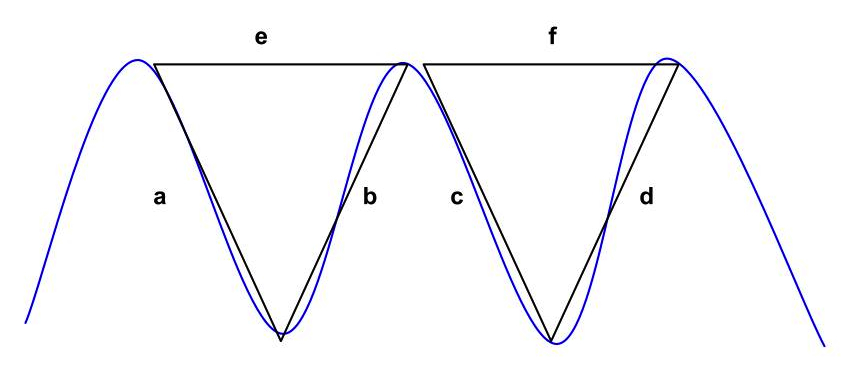
\includegraphics[width=1.05\textwidth]{img/triangles.jpg}
     \caption{}\label{fig:triangles}
\end{figure}
%
\subsubsection{Vertical Oscillation}
%
% TODO: Move this section below 'Overview'
%
The Vertical Oscillation classifier was made to experiment with extracting information from the Optical Flow metadata. It attempts to detect footage where objects in the frames moves up and down, over a period of time. This happens, for example, if people are jumping on the spot, if people close to the camera are gesticulating heavily whilst talking, or if people are thrusting signs into the air. In order to do this we look at the variance of the vertical direction of the optical flow vectors over some time.\\
Like in the Overview classifier we have a set of thresholds, $s$, $t$, and $v$, which are used to regulate the classifier. We start by calculating the standard deviations of the vertical direction of the vectors, throughout the videos. Since the optical flow metadata consists of nine bins of data for each frame, each bin covering one uniuqe ninth of the frame, this is done sepeately for each bin. The parameter $v$ (in our case $v = 12$), determines over how many frames the standard deviation is calculated. Thus, $s$ can be used to determine the frequence of oscillation the classifier should detect. The resulting deviations in each bin are smoothed over 60 frames in order to remove noise, just like in the Overview classifier.
%
% Noter fra Kim: Hvor er den beskrevet (reference + ryk op før vertical oscillation)
%
We then iterate through all frames and for each of them look in each bin to see if the standard deviation in it is above our threshold, $s$. If this is the case for more than $t$ bins, we consider the frame to contain vertical oscillation.
%
% TODO: Little bit more here...
%
\subsubsection{In crowd}
%
We exploited an inherent limitation in facial detection; that faces far away in the image are rarely detected. Due to the nature of our datasets, and we do not try to cover up in any way that this particular label is highly overfitted for this exact purpose, waranted that when multiple faces,
%
% Noter fra Kim: Hvad vil i sige med dette? Pas på blah blah!
%
on average 2 or more faces, are detected we would almost certainly be in a crowd or overlooking a crowd from within.\\
Technically speaking we would compute the moving average over 12 frames (500 ms) of people detected (profile, frontal, or upper body) and if we had detected more than 1 person we would deem that particular frame to be in a crowd.
%
% Noter fra Kim: Hvorfor datid?
%
One must have in mind that there are 24 frames each second, and the facial detection will far from detect (the same) faces/people in each consequtive frame, even for a fairly still image. Hence we had to interpolate the data to get a good estimate.\\
This method could be made even more accurate if we instead of employing a moving average would interpolate each bounding box (bounding the detected object), but also a more complex method.
%
\subsubsection{Person in Focus}
%
The method for detected a person in focus was simple. It works much like the in crowd detection, with the extra constraint that the bounding box of the detected face must be centrally placed in the frame.
%
% Noter fra Kim: Mere detaljer
%
The data was interpolated over 4 frames of a moving average as we wanted a more consistent detection.
%
%
% Noter fra Kim: I skriver stedvist som en dagbog! Hold den akedemiske stil!
%
\subsubsection{Overview}
%
% Noter fra Kim: + Classifier. Flyt afsnit!
%
%
Our Overview classifier attempts to detect footage with little camera movement, little internal movement within the frames, and which is not focusing on any particular single object.
%
% Noter fra Kim: Hvorfor det?
%
It uses the Support Vector Magnitude metadata described in section [SEC:REF], the Optical Flow metadata described in section [SEC:REF], as well as the actual labels classified by the Person in Focus classifier described in section [SEC:REF]. First the Optical Flow data is smoothed over 60 frames (slightly less than 3 seconds) in order to remove noise. The other two sets of metadata have already been smoothed or de-noised during their computation.\\
%
% Noter fra Kim: I bør vel angive klart hvad jeres defininition af Overview shot (er)
%
First we make sure that the frame has not already been classified as containing a Person in Focus, since this goes against our definition of an Overview shot. Now, let $s$, $t$ and $u$ be the threshold that we use to regulate the classifier. We then look at the mean vector length of the optical flow. Since each frame contains nine seperate optical flow means (for different parts of the image), we start by looking at how many of these means are below the threshold $s$. In our case $s=2$ made sense, but different resolutions will require different values. If the number of bins passing the test is larger than $t$ (in our case $7$, meaning that almost the entire image must have very little movement within), we futher make sure that the shift vector magnitude is less than $u$ (again, $10$ made sense in our case, but it will be dependant on resolution).
%
% Noter fra Kim: Mange af jeres variable valg virker sat arbitrært! Kan i dokumentere(?) jeres valg?
%
Only if the frame passes all checks will it be classified with the Overview label.\\
The many different thresholds, as well as the different phases of smoothing, allows for a lot of tweaking. It is also very difficult to test the overall correctness of the classifier, due to the subjectiveness of what makes an Overview shot. Our configuration have been derived through emperical testing and thus may be over-fittet to our specific dataset.
%
\subsubsection{Day \& Night}
%
Our Day \& Night classifier is mostly a proof-of-concept. The time of creation is stored as part of the video file's metadata when it is recorded. As previously explained, this information is stripped away when the video is uploaded to Youtube, but should be available to us in a real scenario. However, Day \& Night classification can actually be done with high accuracy even without this informaton. In [REF] the authors describe how to classify still images through a hierachy of Support Vector Machines, including day/night classification. We have however come up with a much simpler approach, with a very high success rate.\\
Based around the fact that night footage has a significantly less amount of blue compared to footage recorded during the day, we compare the Blue Channel metadata (described in section [SEC:REF]) with the Brightness metadata (described in [SEC:REF]) in order to determine how they correlate. Let $i$ be the frame number in the video, and let $R$ and $L$ be the set of brightness- and \textit{blueness}- values for all frames, respectively. Then the correlation $C_{i}$ is defined as:\\
%
\begin{equation}
C_{i} = \frac{L_{i}}{R_{i}} - 1
\end{equation}
%
A value above zero shows that blue is a dominant color in the frame. The mean of $C$ thus indicates whether the footage is recorded during day- or night- time. Simply using this as a determinant yields a success-ratio of ~88\%, across 301 video clips of various length.
%
% Noter fra Kim: Er det jeres komplette datasæt eller kun træningssættet? Pas på overfitting! metode
% Noter fra Lauge: Flyt disse resultater ned i Results afsnit.  
%
However we can futher look at the general distribution of color intensity we are able to improve this rate further.\\
We start by creating a histogram of the brightness distribution across the entire video. The histograms have a range of [0:255] and contain 10 bins of equal size. For each frame in the video, the mean brightness value is inserted in the histogram. Now we compare the lower
%
% Noter fra Kim: Lower? (beskriv bedre + figur)
%
end of the brightness spectrum
%
% Noter fra Kim: What? Histogram?
%
with the number of frames in the higher end like this:
%
\begin{equation}
\sum_{i=0}^{m}H_{i} < \sum_{j=m+1}^{10}H_{j}
\end{equation}
%
%
% Noter fra Kim: Forklar bedre. Evt. 'Compare the mass in the partitions' + evt. figur
%
Here $H$ is the histogram and $m$ is some value in the range $m\in [1..10]$ (we found $3$ to work quite well). If this statement is true or if the mean of $C$ is above zero we classify the video as day. Otherwise we classify it as night. With this modification we are able to increase the success-rate to ~97\%. And even then, some of the few false classifications that does occur would be difficult to classify manually since they occur in videos recorded in the evening or the late afternoon.
